\chapter{Results}
This chapter present the results of the bachelor thesis. Because a lot of changes
influence the simulation but are not observable, only visible results are mentioned
in this chapter.

\section{Draw sphere cells}
With the created method the program is now able to draw a cell as sphere out of
voxel, as it is displayed in figure 4.1 and 4.2. Since voxels are used in the 3D sim-
ulation, it is not possible to draw a real sphere. Therefore, an approximation to the
volume, surface and the shape is done with these voxels. With this approximation
to a real sphere it is possible to draw cells, which look like spheres.

\begin{figure}
	\begin{center}
	\subfloat[]{
		\hspace{0.5cm}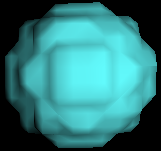
\includegraphics[scale=1.05]{figures/VoxelSphere/Radius5-0.png}
	}
	\subfloat[]{
		\hspace{1cm}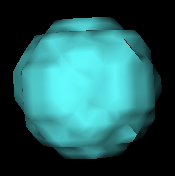
\includegraphics[scale=0.9]{figures/VoxelSphere/Radius5-1.png}
	}
	\end{center}
	\begin{center}
	\subfloat[]{
		\hspace{0.5cm}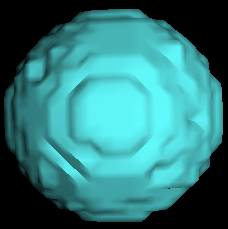
\includegraphics[scale=0.73]{figures/VoxelSphere/Radius9-0.png}
	}
	\subfloat[]{
		\hspace{1cm}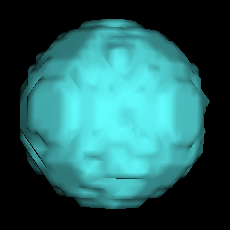
\includegraphics[scale=0.71]{figures/VoxelSphere/Radius9-1.png}
	}
	\end{center}
	\caption{\label{img:DrawnSphereCellRadius5And9}A single cell drawn into the simulation field. The radius of the cell of (a) and (b) is 5 and the radius of the cell of (c) and (d) is 9. Pictures (a) and (c) are with the front view, whereas the
pictures (b) and (d) have an view angle of around 45 degree. The color of the cell is chosen in
a way that more details are visible.}
\end{figure}

\begin{figure}
	\begin{center}
	\subfloat[]{
		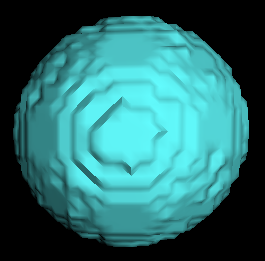
\includegraphics[scale=0.65]{figures/VoxelSphere/Radius14-0.png}
	}
	\subfloat[]{
		\hspace{0.5cm}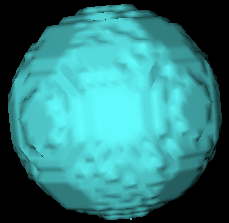
\includegraphics[scale=0.76]{figures/VoxelSphere/Radius14-1.png}
	}
	\end{center}
	\begin{center}
	\subfloat[]{
		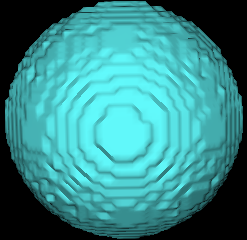
\includegraphics[scale=0.705]{figures/VoxelSphere/Radius23-0.png}
	}
	\subfloat[]{
		\hspace{0.5cm}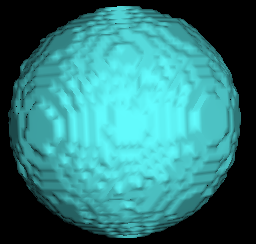
\includegraphics[scale=0.695]{figures/VoxelSphere/Radius23-1.png}
	}
	\end{center}
	\caption{\label{img:DrawnSphereCellRadius5And9}A single cell drawn into the simulation field. The radius of the cell of (a) and (b) is 14 and the radius of the cell of (c) and (d) is 23. Pictures (a) and (c) are with the front view, whereas the
pictures (b) and (d) have an view angle of around 45 degree. The color of the cell is chosen in
a way that more details are visible.}
\end{figure}

Since in the simulation are lattice constraints as well as other cells, it is possible
that the shape of a sphere will not be kept during the simulation. Moreover, the
deviation of the volume and surface between the in pixels drawn and grown sphere
to a real sphere grows as the radius of the sphere grows as it is displayed in figure
XY. A result of a drawn cell with different radius and voxel densities is displayed
at figure xy.



A single cell drawn into the simulation field. The radius of the cell of (a) and (b) is 14 and the
radius of the cell of (c) and (d) is 23. Pictures (a) and (c) are with the front view, whereas the
pictures (b) and (d) have an view angle of around 45 degree. The color of the cell is chosen in
a way that more details are visible.